\documentclass[12pt]{article}
\usepackage{tikz}

\title{Hygienekonzept\\der Studenteninitiative IZ. e.V. (ascii)}
\date{26.11.2020}
\author{}

% hier kommen die Kontaktdaten rein
\newcommand*{\responsibleName}{Max Mustermann}
\newcommand*{\responsibleMail}{muster@mustermail.whatever}
\newcommand*{\responsiblePhone}{+0123456789}

\begin{document}

    \maketitle

    \section*{Grundlagen}

        \begin{itemize}
            \item Sächsische Corona-Schutz-Verordnung in der jeweils gültigen Fassung
            \item Anordnung von Hygieneauflagen in der jeweils gültigen Fassung
            \item Arbeitsschutzstandard des Bundesministeriums für Arbeit und Soziales mit Konkretisierungen der Unfallkasse Sachsen bzw. der brachenspezifischen Berufsgenosseschaften
            \item Hygienekonzept der Fakultät Informatik
        \end{itemize}

    \section*{Verantwortlichkeit}
        \responsibleName \\
        \responsibleMail \\
        \responsiblePhone

    \section{Art der Tätigkeiten, Unterweisung}
        Die Räume APB/E015 und APB/E016 werden genutzt, um den anwesenden Mitarbeitern den Zugang zu Heißgetränken zu ermöglichen.
        Die Mitglieder des Vereins nutzen die Räume auch als Lernumgebung.
        Alle Mitglieder werden durch die Informationen der TU Dresden und den Vorstand von den jeweils geltenden Hygienemaßnahmen unterrichtet.

    \section{Voraussetzungen}
        Voraussetzungen für die Tätigkeiten vor Ort:
        \begin{itemize}
            \item Die Beschäftigten/Besucher bestätigen keine Symptome einer Atemwegserkrankung aufzuweisen und hatten in den letzten 14 Tagen keinen Kontakt zu einer mit SARS-CoV-2 infizierten Person.
            \item Die Kontaktdaten (Name, E-Mail oder Telefonnummer) sind - geschützt vor Einsichtnahme durch Dritte - zu erheben.
            \item Der Verkauf von Getränken richtet sich nach den Regulierungen der Mensa.
        \end{itemize}

    \section{Maßnahmen zur Einhaltung des Mindestabstands von 1,5 m zwischen Personen}
        Bei der Planung sind die jeweils aktuell geltenden rechtlichen Vorgaben zu beachten.
        Die Raumgrößen sind so zu wählen, dass die Abstandsregel von mindestens 1,5 m zwischen Personen sicher eingehalten werden kann.
        \begin{itemize}
            \item Im Gebäude Andreas-Pfitzmann-Baus (APB) tragen alle Personen eine Mund-Nasen-Bedeckung.
            \item Die Einhaltung des Mindestabstands entbindet nicht von derMaskenpflicht.
            \item Am Eingang des Gebäude Andreas-Pfitzmann-Baus und an den Lehrräumen sind Beschilderungen (z.B. Piktogramm) mit Hinweis auf Mindestabstand, Maskenpflicht und Registrierung mittels ZIH-Toolangebracht.
            \item Der Verkauf von Getränken erfolgt durch die Tür. 
                Das Betreten des Raums für nicht Mitglieder ist nicht gestattet. 
                Im Foyer sind Abstandsmarkierungen angebracht.
            \item Maximal 4 Personen aus 2 Hausständen dürfen sich in den Räumen aufhalten. 
        \end{itemize}

        \begin{center}
            \begin{figure}
    \centering
    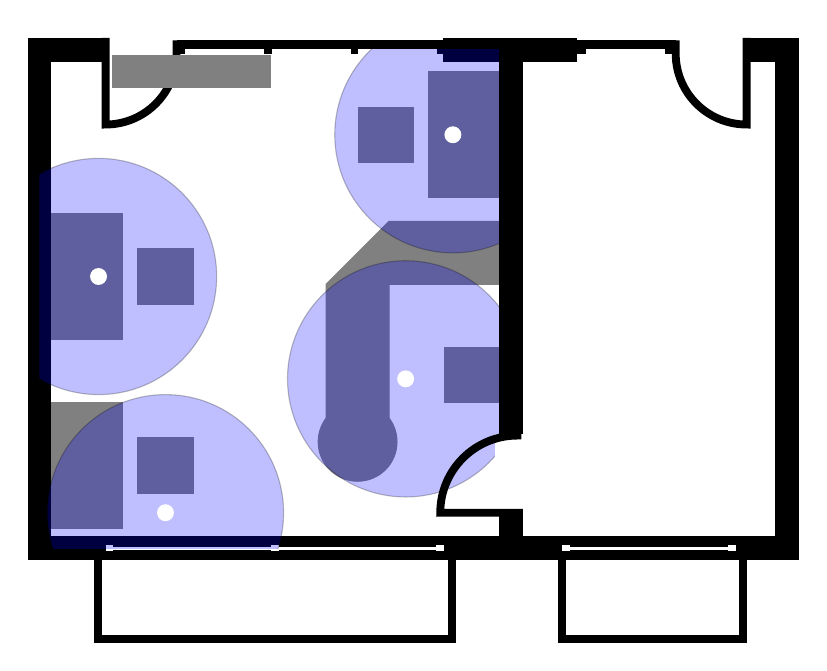
\begin{tikzpicture}[scale=1.0]

        % E016
        \begin{scope}
            % Wand
            \draw [line width=0.3cm] (-0.15,-0.15) rectangle (5.84,6.18);

            % Fenster Foyer
            \draw [color=white, line width=0.20cm] (0.69,6.03) -- (4.98,6.03);
            \draw [color=white, line width=0.16cm] (0.69,6.38) -- (4.98,6.38);

            \draw [color=white, line width=0.32cm] (3.90,6.03) -- (4.90,6.03);
            \draw [color=white, line width=0.32cm] (2.80,6.03) -- (3.80,6.03);
            \draw [color=white, line width=0.32cm] (1.70,6.03) -- (2.70,6.03);

            % Tür Foyer
            \draw [color=white, line width=0.28cm] (0.70,6.18) -- (1.60,6.18);
            \draw [line width=0.1cm] (0.69,6.33) -- (0.69,5.23) arc (90:180:-0.9) -- (1.59,6.30);

            % Fenster Wand
            \draw[color=white, line width=0.04cm] (0.69,-0.15) -- (4.99,-0.15);
            \draw[line width=0.1cm] (0.59,-0.3) -- (0.59,-1.3) -- (5.09,-1.3) -- (5.09,-0.3);
            \draw[color=white, line width=0.08cm] (0.69,-0.15) -- (0.79,-0.15);
            \draw[color=white, line width=0.08cm] (2.79,-0.15) -- (2.89,-0.15);
            \draw[color=white, line width=0.08cm] (4.89,-0.15) -- (4.99,-0.15);
        \end{scope}

        % E016 Möbel
        \begin{scope}[color=gray]
            % Theke
            \draw[fill=gray] (5.69,4.00) -- (4.29,4.00) -- (3.49,3.20) -- (3.49,1.00) -- (4.29,1.00) -- (4.29,3.20) -- (5.69,3.20);
            \draw[fill=gray] (5.69,1.70) rectangle (4.99,2.40);
            \draw[fill=gray] (3.89,1.20) circle (0.5);

            % Tisch Fenster
            \draw[fill=gray] (0.78,6.1) rectangle (2.78,5.7);

            % Sofa oben rechts
            \draw[fill=gray] (5.69,5.9) rectangle(4.79,4.3);
            \draw[fill=gray] (4.6,5.45) rectangle (3.9,4.75);

            % Sofa unten links
            \draw[fill=gray] (0.00,0.10) rectangle (0.90,1.70);
            \draw[fill=gray] (1.1,0.55) rectangle (1.8,1.25);

            % Sofa mitte links
            \draw[fill=gray] (0.00, 2.50) rectangle (0.90,4.10);
            \draw[fill=gray] (1.1,2.95) rectangle (1.8,3.65);
        \end{scope}

        % Corona
        \begin{scope}
            \clip (-0.15,-0.15) rectangle (5.84,6.18);

            % Theke
            \draw[fill=blue, opacity=0.25] (4.5,2.0) circle (1.5);
            \draw[fill=white, color=white] (4.5,2.0) circle (0.1);

            % Sofa oben rechts
            \draw[fill=blue, opacity=0.25] (5.1,5.1) circle (1.5);
            \draw[fill=white, color=white] (5.1,5.1) circle (0.1);
            
            % Sofa unten links
            \draw[fill=blue, opacity=0.25] (1.45,0.3) circle (1.5);
            \draw[fill=white, color=white] (1.45,0.3) circle (0.1);
            
            % Sofa mitte links
            \draw[fill=blue, opacity=0.25] (0.6,3.3) circle (1.5);
            \draw[fill=white, color=white] (0.6,3.3) circle (0.1);
        \end{scope}

        % E015
        \begin{scope}[shift={(5.99,0)}]
            % Wand
            \draw [line width=0.3cm] (-0.15,-0.15) rectangle (3.35,6.18);

            % Fenster Foyer
            \draw [color=white, line width=0.20cm] (0.69,6.03) -- (2.84,6.03);
            \draw [color=white, line width=0.16cm] (0.69,6.38) -- (2.84,6.38);

            \draw [color=white, line width=0.32cm] (0.80,6.03) -- (1.80,6.03);

            % Tür Foyer
            \draw [color=white, line width=0.28cm] (1.94,6.18) -- (2.84,6.18);
            \draw [line width=0.1cm] (2.84,6.33) -- (2.84,5.23) arc (270:180:0.9) -- (1.94,6.30);

            % Tür Lager
            \draw [color=white, line width=0.4cm] (-0.15, 0.30) -- (-0.15,1.30);
            \draw [line width=0.1cm] (0.0,0.30) -- (-1.05, 0.30) arc (0:-90:-0.98) -- (-0.07,1.30);

            % Fenster Wand
            \draw[color=white, line width=0.04cm] (0.6,-0.15) -- (2.7,-0.15);
            \draw[line width=0.1cm] (0.5,-0.3) -- (0.5,-1.3)  -- (2.8,-1.3)-- (2.8,-0.15);
            \draw[color=white, line width=0.08cm] (0.5,-0.15) -- (0.6,-0.15);
            \draw[color=white, line width=0.08cm] (2.6,-0.15) -- (2.7,-0.15);
        \end{scope}
    \end{tikzpicture}
\end{figure}

        \end{center}

    \section{Hygienemaßnahmen}
        \begin{itemize}
            \item Alle Personen (Beschäftigte und Besucher) haben eine Mund-Nasen-Bedeckung im Gebäude zutragen.
            \item Alle Personen (Beschäftigte und Besucher) müssen sich vor dem Betreten von Gebäuden mittels des ZIH-Toolsregistrieren.
            \item Der Besucher-und Publikumsverkehr wird auf ein absolutes Minimumreduzieren.
            \item Besucher haben eine eigene Mund-Nasen-Bedeckungmitzubringen.
            \item Waschgelegenheiten mit Flüssigseife und Einmalpapierhandtüchern sowie Entsorgungsmöglichkeit für Einmalhandtücher sowie Händedesinfektionsmittel stehen in den Waschräumen/Toiletten/E015 des APB zurVerfügung.
            \item Geschirr wird mit einer professionellen Spülmaschine gereinigt.
            \item Alle Arbeitsflächen und Arbeitsmittel werden regelmäßig desinfiziert.
        \end{itemize}

    \section{Anforderungen an Lüftung}
        \begin{itemize}
            \item Die regelmäßige Lüftung vor, während und nach jeder Benutzung von Räumen im APB wird durchgesetzt (abhängig von Personenzahl und Raumgröße: Hilfestellung z.B. durch CO2-App der DGUV für Smartphones ``CO2-Timer'').
            \item Die Räume werden durchgehend mit dem Foyer gelüftet.
        \end{itemize}

\end{document}